\documentclass[a4paper,10pt]{article}
\usepackage[margin=0.5in]{geometry}
\usepackage[utf8]{inputenc}
\usepackage{amsmath}    % need for subequations
\usepackage{graphicx}   % need for figures
\usepackage{verbatim}   % useful for program listings
\usepackage{color}      % use if color is used in text
  % use for side-by-side figures
\usepackage{hyperref}  
%opening
\title{Knowledge and Women}
\author{}

\begin{document}

\maketitle

\begin{abstract}
Since ancient times, women have been held at an esteemed position in terms of knowledge. This paper tries to address the role of women who have raised the scientific levels to great heights both from the Western and Indian Perspective. From the western viewpoint,  there has been evidences of Greeks and Romans worshipping Goddess Athena and Minerva, respectively. On a similar note, Indians have regarded Goddess Saraswati as the mother of knowledge and wisdom. The intellectual calibre of Indian women has been explicitly stated in the epics and puranas. For example, there is a mention in Mahabharata indicating the managerial capabilities of Draupadi. These characters, albeit mythological portray the essence of the limitless capabilities of women.

Starting from the historic times, the western world has seen women professionals. Some of them are Merit-Ptah the first known physician from Ancient Egypt, Agamede the first female healer from Greece, Hypatia first known woman mathematician, Charlotta Frolich first female historian,  Marie Curie first woman to win a nobel prize, Laura Bassi first woman to earn a university chair (18th century),  Ada Lovelace first woman programmer, Grace Hopper woman who invented first compiler and Mary Anning Paleontologist.

A few remarkable Indians are Avvaiyar, who was one of the greatest poets of all times,  Gargi and Maithreyi, who are mentioned in the Upanishad texts,  the saint poet Mirabhai, Leelavathi, the mathematician and astrologer, Razia Sultana a monarch, the south asian physicians Kadambini Ganguly and Anandhi Gopal Joshi, the meteorologist Anna Manni, Sarla Takral who was the first woman to fly an aircraft and in the present scenario Dr. Shantha, who is heading the Adayar Cancer Institute. 

This paper explores the effort and dedication put forth by the aforementioned personalities with a hope that it will create an inspiration to the present generation female individuals
\end{abstract}
\section{Introduction}
\section{Case-Studies}

\subsection{Historical Period}
In Vedic period, three Goddesses namely, Illa, Saraswati and Mahi has been quoted for the purpose of acquiring knowledge as \cite{saras}: 

“May Bharati come speeding to our sacrifice and Ila hither awakening our consciousness in human wise, and Saraswati, — three goddesses sit on this blissful seat, doing well the
Work.” 
The image of Goddess (Figure 1) portrays a musical instrument called Veena holding in  two hands, a book in one hand and a tiny garland in another hand. These represent music, knowledge and inner bliss, respectively. 
\begin{center}
\begin{figure}[h]
\centering
 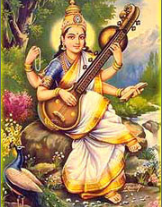
\includegraphics[scale=0.7]{saraswati.png}
 \caption{Goddess Sarawati}
\end{figure}
\end{center}

The Vedic period has seen intellectuals like Gargi and Maithreyi. Gargi Vachnaknavi, who lived during 700 BC was honored as a great philosopher \cite{Gargi}. The debate between Gargi and Yajnavalkya has been specified in Brihadaranyaka Upanishad, in which Gargi puts forth a series of thought provoking questions to Yajnavalkya. A few such questions from this debate is given below. \\


\textit{Yajnavalkya ,`` said she, ``if all this is pervaded by water, by  what, pray, is water pervaded?''} \\
\textit{``By air, O Gargi.", replied Yajnavalkya.} \\
\textit{``By what, pray, is air pervaded?" }\\
\textit{``By the sky, O Gargi."} \\
\textit{``By what is the sky pervaded?"}  \\

These questions clearly indicate scientific thought process of Indian Women. 

On a similar front, in the Indian Epic Mahabharatha, there are instances of women empowerment. Draupadi is known to have managed the people and wealth in the palace \cite{mahabharatha}. 

In South India, around First or Second Century A.D. there was a Tamil Poet called Avvaiyaar. She can be considered as one of the pioneers in Science also, because she specifies about the information of energy of atom in one of her poems as: \\
\begin{center}
``aNuvaith thuLaiththu Ez kadalai puguththi'' \\
\textit{Energy of seven seas within a pierced atom}\\
\end{center}
\newblock
According to the Greek Mythology, Athena is the embodiment of wisdom and power.\\
Various poems written for her by Odysseus G. Osborne spot light the depth of powers that the Goddess has.\\
\begin{center}
\begin{figure}[h]
\centering
 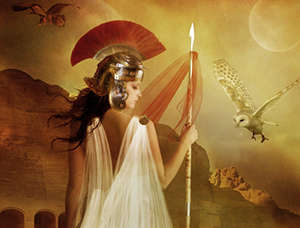
\includegraphics[scale=0.7]{athena_7.jpg}
 \caption{Goddess Sarawati}
\end{figure}
\end{center}

One of the many poems written on Athena in relation to Wisdom as \cite{athena}:\\


\textit{Marshal of Wisdom}\\
\textit{give the gift as you resolve,}\\
\textit{As a Lance of Glory,}\\
\textit{Heralding your puissant strike!}\\
\textit{Or like a silent owl}\\
\textit{A glide on the Nights wind}\\
\textit{With talons wide!}\\
\textit{Mighty Athena! Let me be re-born of your thunderbolt!}\\

\newblock
Minerva was the Roman Goddess of Wisdom and war. She is believed to be the inventor of numbers and musical instruments. She was later equated with the Greek Goddess of Wisdom, Athena.

She was called as the “goddess of thousand works” by Ovid, a Roman poet. She was being worshipped on the Capitoline Hill along with Jupiter and Juno as the Powerful triad of Gods.

\subsection{Medieval Period}
\newblock
Merit-Ptah is believed by Egytologists to be the first-ever named Physician. She is most notable for being the first woman known by name in the history of the field of medicine, and also the first named woman in all of science as well.\\

She practiced medicine nearly 5,000 years ago, and was immortalized by her son on her tomb as “the chief physician”\cite{merit}.
\begin{center}
\begin{figure}[h]
\centering
 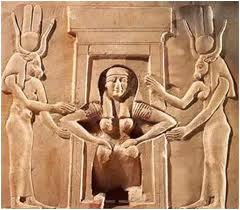
\includegraphics[scale=0.7]{meritptah.jpg}
 \caption{Merit Ptah}
\end{figure}
\end{center}

\newblock
Mythologically According to Homer, Agamede was, according to Homer, a Greek physician acquainted with the healing powers of all the plants that grow upon the earth.\\

\newblock
Agnodike was the first female Athenian physician, midwife, gynaecologist. She studied in Alexandria under the great Herophilos, the first anotomist.

\begin{center}
\begin{figure}[h]
\centering
 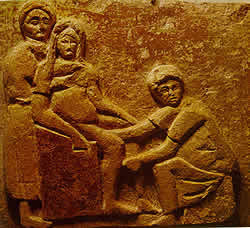
\includegraphics[scale=0.7]{agnodice.jpg}
 \caption{Agnodike}
\end{figure}
\end{center}

\newblock
Maria the Jewess is the first female alchemist and is credited with the invention of several chemaical apparatus.

\newblock
\\Hypatia was a Greek mathematician, astronomer and philosopher in Egypt. She was the head of Neoplatonic school of Alexandria. Her contributions are considered as invention of the hydrometer used to determine the relative density (or specific gravity) of liquids. She worked collaboratively with her father on many works.\\

\subsection{Modern Period}

\newblock
Christine de Pizan is a fifteenth-century writer in France. She is the author of the Book of the City of the Ladies. She was an early feminist who challenged her culture's stereotypes of women.She wrote love ballads, books supporting and extolling the powers and virtues of women (including a response to Jean de Meun's Roman de la rose), and a work about Joan of Arc.\cite{christine}\\

\begin{center}
\begin{figure}[h]
\centering
 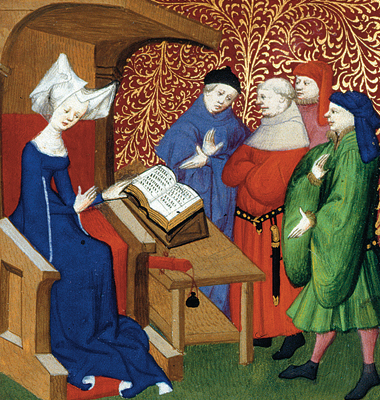
\includegraphics[scale=0.7]{christine.jpg}
 \caption{Christine de Pizan}
\end{figure}
\end{center}

\newblock
\\
Maria Sibylla Merian was a Naturalist, an Entymologist and a Botanical Illustrator.


\begin{center}
\begin{figure}[h]
\centering
 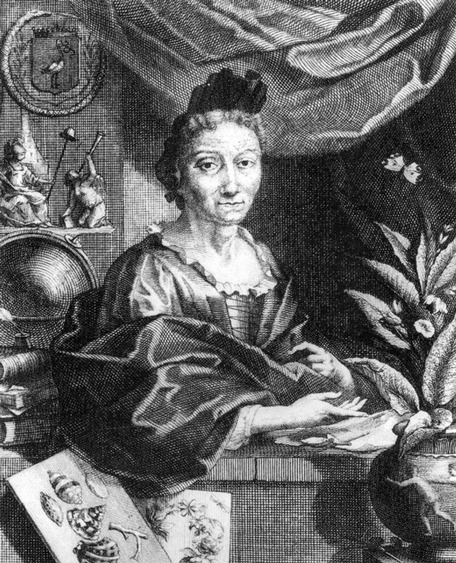
\includegraphics[scale=0.7]{maria.jpg}
 \caption{Maria Sibylla Merian}
\end{figure}
\end{center}


\subsection{Current Era}
\section{Analysis}
\section{Conclusion}
\begin{thebibliography}{9}

\bibitem{sara}
http://www.universityofhumanunity.org/biblios/Sarasvati%20in%20the%20Veda%20-%20Part%201.pdf

\bibitem{Gargi}
Ahuja, M.L. 
\newblock {2011.}
\newblock { Women in Indian Mythology}
\newblock {Rupa Publications}

\bibitem{mahabharatha}
 Kisari Mohan Ganguli
\newblock{The Mahabharata of Krishna-Dwaipayana Vyasa}
\newblock{Translation from original Sanskrit Text}
\newblock{http://sacred-texts.com/hin/maha/index.htm}

\bibitem{athena}
https://sites.google.com/site/shrineathenapromachos/prayers-poems

\bibitem{merit}
http://www.ancient.eu/article/49/

\bibitem{christine}
http://historymedren.about.com/od/cwho/a/Christine-De-Pizan-Quotes.htm

\end{thebibliography}

\end{document}
